\documentclass[12pt]{article}

\usepackage[margin=0.85in]{geometry}
\usepackage{enumitem}
\usepackage{titlesec}
\usepackage{setspace}
\usepackage{amsmath, amssymb}
\usepackage{fancyhdr}
\usepackage{xcolor}
\usepackage{hyperref}
\usepackage{enumitem}
\usepackage{setspace}
\usepackage{amsmath,amssymb}
\usepackage{tikz}

\usetikzlibrary{positioning,arrows.meta}

\DeclareMathOperator*{\argmax}{arg\,max}

\setlength{\parindent}{0pt}

\setstretch{0.97}

\setlength{\parskip}{0pt}

\setlength{\abovedisplayskip}{5pt}
\setlength{\belowdisplayskip}{5pt}

\titlespacing*{\section}{0pt}{0.6em}{0.3em}

\pagestyle{fancy}
\fancyhf{}
\fancyhead[L]{\textbf{ECE 533}}
\fancyhead[C]{\textbf{Final Exam}}
\fancyhead[R]{\textbf{Scott Nguyen}}
\fancyfoot[C]{\thepage}
\renewcommand{\headrulewidth}{0.4pt}

\begin{document}
	
	\begin{center}
		{\Huge \textbf{ECE 533 Final Exam 2026}}\\
		Assigned: Saturday Morning, May 9th, 7 am, 2026.\\
		Due: Sunday, May 10th, Midnight, 2026.\\
		You must submit your final exam online.\\
		\textbf{No collaboration is allowed.}\\
		\textbf{You must direct all questions to the instructor ONLY.}\\
		\textbf{The contribution of the final exam to your final grade will be calculated based}\\
		\textbf{on the syllabus.}
	\end{center}
	
	\section{Grading}
	
	You will receive zero credit if your answers appear to be AI-generated. During grading, I
	will try to assess your understanding of the material as opposed to text that appears to be
	AI-generated. The credit is \textbf{not} distributed equally among problems.
	
	We will meet at our usual time at 9 am for review. The Zoom link for the review is
	\href{https://unm.zoom.us/j/92205338944}{https://unm.zoom.us/j/92205338944}.
	After the review, I will upload the Zoom recording to the assignment link. In other words,
	in order to access the recording, you will need to login in the same place where you
	downloaded the final exam.
	
	After Monday, I will send everyone information about the final project.
	
	\newpage
	
	\noindent\textbf{Problem \#1. The cross-entropy loss function (10 points).}
	
	\noindent The expression for the cross-entropy function is given by:
	
	\[
	J(\Theta)
	=
	-\frac{1}{m}
	\sum_{i=1}^{m}
	\sum_{k=1}^{K}
	y_k^{(i)}
	\log\left(
	\hat{p}_k^{(i)}(\Theta)
	\right)
	\]
	
	where $\Theta$ denotes the parameters learned by the network. Here, $k$ is an index for
	each of the $K$ possible classes, $i$ refers to the $i$-th sample in a batch of $m$ samples,
	$y_k^{(i)}$ is the ground truth for the $k$-th class for the $i$-th sample. Based on the
	learned parameters, $\hat{p}_k^{(i)}$ denotes the estimated probability estimated by the
	network for the $i$-th sample belonging to the $k$-th class. Note that $0\log(0)=0$ as it
	can be shown by L'Hopital's rule.
	
	For each case below, you need to provide:
	
	\begin{enumerate}
		\item ground truth vectors.
		
		\item probability values (not necessarily ideal) to be learned by the network.
		
		\item cross-entropy value.
	\end{enumerate}
	
	Consider the following cases:
	
	\begin{enumerate}
		\item[(i)] All samples belong to the first class. For this case, assume that we have ideal probabilities that need to be learned by the network. In this case, we also get the ideal entropy.
		
		\item[(ii)] A balanced dataset is given. For this case, assume that we have ideal probabilities that need to be learned by the network. What is the requirement for $m$ so as to have a balanced dataset in each batch?
		
		\item[(iii)] A balanced dataset is given. For this case, assume two classes. Initially, prior to learning, the probabilities are at their worst. You need to give the worst possible probabilities for this case and the corresponding cross-entropy value.
	\end{enumerate}
	
	\textbf{Solution}
	
	\begin{enumerate}[itemsep=2pt]
		
		\item[(i)] Since all samples belong to the first class, the ground-truth vector for every sample is
		
		\[
		y^{(i)} = [1,0,\ldots,0]
		\]
		
		In the ideal case, the network predicts
		
		\[
		\hat{p}^{(i)} = [1,0,\ldots,0]
		\]
		
		Since the correct class probability is 1,
		
		\[
		-\log(1)=0
		\]
		
		Therefore,
		
		\[
		J(\Theta)=0
		\]
		
		\item[(ii)] For a balanced dataset with \(K\) classes, the batch size \(m\) must satisfy
		
		\[
		m \bmod K = 0
		\]
		
		so each class appears equally often. The ground-truth vectors are one-hot encoded, and in the ideal case the predicted probabilities match them exactly:
		
		\[
		y^{(i)}=[1,0,0]
		\qquad
		\hat{p}^{(i)}=[1,0,0]
		\]
		
		Therefore,
		
		\[
		J(\Theta)=0
		\]
		
		\item[(iii)] For a balanced dataset with two classes, the worst prediction occurs when the network assigns probability 0 to the correct class and 1 to the incorrect class:
		
		\[
		y^{(i)}=[1,0]
		\qquad
		\hat{p}^{(i)}=[0,1]
		\]
		
		\[
		y^{(i)}=[0,1]
		\qquad
		\hat{p}^{(i)}=[1,0]
		\]
		
		In this case,
		
		\[
		-\log(0)\rightarrow\infty
		\]
		
		Therefore, the cross-entropy loss approaches infinity.
		
	\end{enumerate}
	
	\newpage
	
	\noindent\textbf{Problem \#2. Binary Loss functions (15 points).}
	
	\noindent\textbf{2(a)} Recall the logistic regression loss function:
	
	\[
	J(\theta)
	=
	-\frac{1}{m}
	\sum_{i=1}^{m}
	\left[
	y^{(i)}\log\left(p^{(i)}\right)
	+
	\left(1-y^{(i)}\right)\log\left(1-p^{(i)}\right)
	\right]
	\]
	
	Here, \(p^{(i)}\) is the predicted probability and \(y^{(i)}\) is the ground-truth label for the \(i\)-th sample.
	
	Assume that an object is classified as positive when the positive probability is \(>0.5\). For each case below, provide values for all symbols in the loss function.
	
	\begin{enumerate}[itemsep=2pt]
		\item[(i)] A true positive with a positive classification probability of \(0.9\).
		
		\item[(ii)] A false positive with a negative classification probability of \(0.3\).
		
		\item[(iii)] A true negative with a positive classification probability of \(0.2\).
		
		\item[(iv)] A false negative with a positive classification probability of \(0.45\).
	\end{enumerate}
	
	\vspace{0.2cm}
	
	\noindent\textbf{Solution}
	
	\begin{enumerate}[itemsep=2pt]
		
		\item[(i)] True positive:
		
		\[
		y^{(i)}=1
		\qquad
		p^{(i)}=0.9
		\]
		
		\[
		J(\theta)=-\log(0.9)
		\]
		
		\item[(ii)] False positive:
		
		\[
		y^{(i)}=0
		\qquad
		p^{(i)}=0.7
		\]
		
		since the negative probability is \(0.3\).
		
		\[
		J(\theta)=-\log(0.3)
		\]
		
		\item[(iii)] True negative:
		
		\[
		y^{(i)}=0
		\qquad
		p^{(i)}=0.2
		\]
		
		\[
		J(\theta)=-\log(0.8)
		\]
		
		\item[(iv)] False negative:
		
		\[
		y^{(i)}=1
		\qquad
		p^{(i)}=0.45
		\]
		
		\[
		J(\theta)=-\log(0.45)
		\]
		
	\end{enumerate}
	
	\newpage
	
	\noindent\textbf{2(b)} We often get an imbalanced dataset, and we are asked to use weighting factors to rebalance the error. For example, for two classes, if we have 10 times as many samples in class 0, we would multiply the error for class 1 by 10. Provide the modified loss function for this case. This problem refers to the cross-entropy function (see Problem 1).
	
	\vspace{0.2cm}
	
	\noindent\textbf{Solution}
	
	For a weighted binary cross-entropy loss, a weighting factor is added to increase the penalty for the minority class. Since class 1 has fewer samples, its error term is multiplied by 10:
	
	\[
	J(\theta)
	=
	-\frac{1}{m}
	\sum_{i=1}^{m}
	\left[
	10\,y^{(i)}\log\left(p^{(i)}\right)
	+
	\left(1-y^{(i)}\right)\log\left(1-p^{(i)}\right)
	\right]
	\]
	
	This increases the contribution of class 1 errors during training and helps rebalance the learning process.
	
	\newpage
	
	\noindent\textbf{2(c)} Generalize your answer in 2(b) for K classes. This problem refers to the cross-entropy function (see Problem 1).
	
	\vspace{0.2cm}
	
	\noindent\textbf{Solution}
	
	For \(K\) classes, a separate weighting factor \(w_k\) is assigned to each class to account for class imbalance. The weighted cross-entropy loss becomes
	
	\[
	J(\Theta)
	=
	-\frac{1}{m}
	\sum_{i=1}^{m}
	\sum_{k=1}^{K}
	w_k\,y_k^{(i)}
	\log\left(\hat{p}_k^{(i)}\right)
	\]
	
	where \(w_k\) is the weight associated with class \(k\). Larger weights are assigned to minority classes so that their errors contribute more strongly during training.
	
	\newpage
	
	\noindent\textbf{Problem \#3. Basics of Stochastic Gradient Descent (10 points).}
	
	\noindent\textbf{3(a)} Consider the following relates model that relates the inputs to the outputs:
	
	\[
	\hat{y}^{(i)} = a \cdot x_{(i)}^2 + b \cdot x_{(i)} + c
	\]
	
	where \(i\) refers to the \(i\)-th sample, \(\hat{y}^{(i)}\) refers to the estimated ground truth for the \(i\)-th sample, \(x_{(i)}\) refers to the input value, and \(a,b\) refer to the model parameters.
	
	To implement stochastic gradient descent (SGD), we identify that we need to estimate the parameters
	
	\[
	\theta = (a,b,c).
	\]
	
	In order to estimate \(\theta\), we consider the mean-squared error as a loss function given by:
	
	\[
	\mathrm{MSE}
	=
	\frac{1}{N}
	\sum_{i=1}^{i=N}
	\left(
	y^{(i)}-\hat{y}^{(i)}
	\right)^2 .
	\]
	
	In SGD, instead of evaluating the whole sum, we simply evaluate the error at a single sample:
	
	\[
	\mathrm{MSE}_1
	=
	\left(
	y^{(i)}-\hat{y}^{(i)}
	\right)^2 .
	\]
	
	Compute the gradient of the single-sample error by substituting the expression for \(\hat{y}^{(i)}\) and taking the partial derivatives:
	
	\[
	\frac{\partial}{\partial a}\mathrm{MSE}_1,
	\quad
	\frac{\partial}{\partial b}\mathrm{MSE}_1,
	\quad
	\text{and}
	\quad
	\frac{\partial}{\partial c}\mathrm{MSE}_1 .
	\]
	
	Then provide the final expression for the gradient using:
	
	\[
	\nabla_{\theta}\ \mathrm{MSE}_1
	=
	\left(
	\frac{\partial}{\partial a}\mathrm{MSE}_1,
	\frac{\partial}{\partial b}\mathrm{MSE}_1,
	\frac{\partial}{\partial c}\mathrm{MSE}_1
	\right).
	\]
	
	\textbf{Hint:} While the notation may look intimidating, this is a very simple derivative problem. The following part is also simple because it asks you to evaluate the derivative at a point.

	\vspace{0.2cm}
	
	\noindent\textbf{Solution}
	
	First, substitute the expression for \(\hat{y}^{(i)}\) into the single-sample error:
	
	\[
	\mathrm{MSE}_1
	=
	\left(
	y^{(i)}
	-
	\left(
	a\,x_{(i)}^2+b\,x_{(i)}+c
	\right)
	\right)^2
	\]
	
	Using the chain rule, the partial derivatives are:
	
	\[
	\frac{\partial}{\partial a}\mathrm{MSE}_1
	=
	-2x_{(i)}^2
	\left(
	y^{(i)}-\hat{y}^{(i)}
	\right)
	\]
	
	\[
	\frac{\partial}{\partial b}\mathrm{MSE}_1
	=
	-2x_{(i)}
	\left(
	y^{(i)}-\hat{y}^{(i)}
	\right)
	\]
	
	\[
	\frac{\partial}{\partial c}\mathrm{MSE}_1
	=
	-2
	\left(
	y^{(i)}-\hat{y}^{(i)}
	\right)
	\]
	
	Therefore, the gradient vector is
	
	\[
	\nabla_{\theta}\mathrm{MSE}_1
	=
	\left(
	-2x_{(i)}^2(y^{(i)}-\hat{y}^{(i)}),
	\,
	-2x_{(i)}(y^{(i)}-\hat{y}^{(i)}),
	\,
	-2(y^{(i)}-\hat{y}^{(i)})
	\right)
	\]
	
	\newpage
	
	\noindent\textbf{3(b)} We present the modified stochastic gradient descent (SGD) algorithm below. It uses \(\mathrm{MSE}_1\) to search for a solution. In what follows, we will investigate a few steps of the algorithm.
	
	\begin{flushleft}
		Initialize $\theta=(a,b,c)$ using random sampling.
		
		\textbf{for} epoch$=1$ to NumOfEpochs
		
		\hspace*{1cm}\textbf{for} sample$=1$ to NumOfTrainSamples
		
		\hspace*{2cm}Select $i$ using random sampling
		
		\hspace*{2cm}\textbf{Compute weights gradient using }$(x_i,y_i)$:
		
		\hspace*{3cm}$g=\nabla_{\theta}\ \mathrm{MSE}_1$
		
		\hspace*{2cm}\textbf{Compute learning rate:}
		
		\hspace*{3cm}$\eta=f(\mathrm{epoch},\mathrm{sample})$
		
		\hspace*{2cm}\textbf{Update weights using gradient:}
		
		\hspace*{3cm}$\theta=\theta-\eta\cdot g$
	\end{flushleft}
	
	In this part, we will trace the application of the algorithm. After random sampling, we set an initial value for
	
	\[
	\theta=(a,b,c)=(1,2,5).
	\]
	
	For the first epoch, suppose that we randomly sample \(i=3\) and we pick the pair \((x_3,y_3)\). For this case, let \(y_3\) denote the ideal value for \(x_3=3\). Assume that
	
	\[
	\eta=1e^{-6},
	\]
	
	and provide an estimate for \(\theta\) by applying
	
	\[
	\theta=\theta-\eta\cdot g.
	\]
	
	\noindent\textbf{Solution}
	
	For the sampled point, we have
	
	\[
	x_3=3
	\]
	
	and the current parameter vector is
	
	\[
	\theta=(a,b,c)=(1,2,5).
	\]
	
	Using the model,
	
	\[
	\hat{y}^{(3)}
	=
	a\,x_3^2+b\,x_3+c
	\]
	
	we obtain
	
	\[
	\hat{y}^{(3)}
	=
	1(3^2)+2(3)+5
	=
	9+6+5
	=
	20.
	\]
	
	Since \(y_3\) is the ideal value for \(x_3=3\), the error term is
	
	\[
	y_3-\hat{y}^{(3)}
	=
	3-20
	=
	-17.
	\]
	
	Using the gradient expressions from Part 3(a):
	
	\[
	\frac{\partial}{\partial a}\mathrm{MSE}_1
	=
	-2(3^2)(-17)
	=
	306
	\]
	
	\[
	\frac{\partial}{\partial b}\mathrm{MSE}_1
	=
	-2(3)(-17)
	=
	102
	\]
	
	\[
	\frac{\partial}{\partial c}\mathrm{MSE}_1
	=
	-2(-17)
	=
	34
	\]
	
	Therefore,
	
	\[
	g=(306,102,34).
	\]
	
	Using
	
	\[
	\eta=10^{-6},
	\]
	
	the parameter update becomes
	
	\[
	\theta
	=
	\theta-\eta g
	\]
	
	\[
	\theta
	=
	(1,2,5)-10^{-6}(306,102,34)
	\]
	
	\[
	\theta
	=
	(0.999694,\ 1.999898,\ 4.999966).
	\]
		
	\newpage
	
	\noindent\textbf{Problem \#4. SoftMax and dot products (20 points).}
	
	For the SoftMax layer, we learn parameters \(\theta^{(k)}\). Then we compute dot products against the input vectors given by
	
	\[
	s_k(\mathbf{x})
	=
	(\theta^{(k)})^T\mathbf{x}.
	\]
	
	The probabilities for each class are given by the softmax function:
	
	\[
	\hat{p}_k
	=
	\sigma(\mathbf{s}(\mathbf{x}))_k
	=
	\frac{\exp(s_k(\mathbf{x}))}
	{\sum_{j=1}^{K}\exp(s_j(\mathbf{x}))}.
	\]
	
	We classify the input based on the class that maximizes \(\hat{p}_k\) as given by:
	
	\[
	\hat{y}
	=
	\argmax_k\ \sigma(\mathbf{s}(\mathbf{x}))_k
	=
	\argmax_k\ s_k(\mathbf{x})
	=
	\argmax_k\ \left((\theta^{(k)})^T\mathbf{x}\right)
	\]
	
	In what follows, we will consider the case of two classes.
	
	\newpage
	
	\noindent\textbf{4(a)} For each of the following cases, sketch how the 2-D input vectors \(\mathbf{x}\) will get classified into class 1 or class 2:
	
	\begin{enumerate}[itemsep=6pt]
		
		\item[(i)]
		\[
		\theta^{(1)}=[1,2]^T,
		\quad
		\theta^{(2)}=[-1,2]^T
		\]
		
		\item[(ii)]
		\[
		\theta^{(1)}=[1,5]^T,
		\quad
		\theta^{(2)}=[5,-1]^T
		\]
		
		\item[(iii)]
		\[
		\theta^{(1)}=[1,2]^T,
		\quad
		\theta^{(2)}=[2,4]^T
		\]
		
	\end{enumerate}
	
	For full credit, you need to show:
	
	\begin{enumerate}[itemsep=6pt]
		
		\item[(a)] all decision vectors plotted.
		
		\item[(b)] shaded region on the 2D plane for each class.
		
		\item[(c)] boundary (if any) between the two classes.
		
	\end{enumerate}
	
	\noindent\textbf{Solution}
	
	A point \(\mathbf{x}=[x_1,x_2]^T\) is classified by comparing
	\[
	(\theta^{(1)})^T\mathbf{x}
	\quad \text{and} \quad
	(\theta^{(2)})^T\mathbf{x}.
	\]
	The decision boundary occurs when
	\[
	(\theta^{(1)}-\theta^{(2)})^T\mathbf{x}=0.
	\]
	
	\begin{enumerate}[itemsep=8pt]
		
		\item[(i)] 
		\[
		\theta^{(1)}-\theta^{(2)}=[1,2]^T-[-1,2]^T=[2,0]^T
		\]
		so the boundary is
		\[
		2x_1=0 \Rightarrow x_1=0.
		\]
		Class 1 occurs when \(x_1>0\), and class 2 occurs when \(x_1<0\).
		
		\begin{center}
			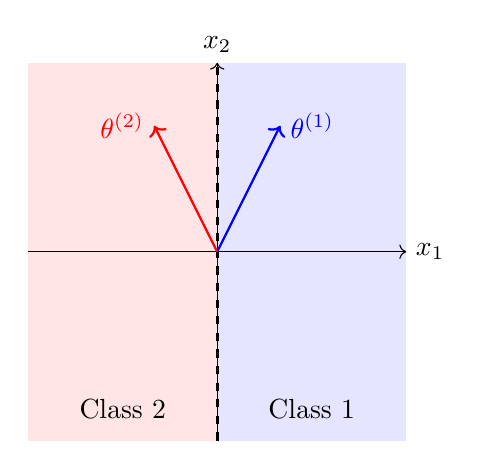
\begin{tikzpicture}[scale=0.8]
				\fill[blue!10] (0,-3) rectangle (3,3);
				\fill[red!10] (-3,-3) rectangle (0,3);
				
				\draw[->] (-3,0) -- (3,0) node[right] {$x_1$};
				\draw[->] (0,-3) -- (0,3) node[above] {$x_2$};
				
				\draw[very thick, dashed] (0,-3) -- (0,3);
				
				\draw[->, thick, blue] (0,0) -- (1,2) node[right] {$\theta^{(1)}$};
				\draw[->, thick, red] (0,0) -- (-1,2) node[left] {$\theta^{(2)}$};
				
				\node at (1.5,-2.5) {Class 1};
				\node at (-1.5,-2.5) {Class 2};
			\end{tikzpicture}
		\end{center}
		
		\item[(ii)]
		\[
		\theta^{(1)}-\theta^{(2)}=[1,5]^T-[5,-1]^T=[-4,6]^T
		\]
		so the boundary is
		\[
		-4x_1+6x_2=0
		\Rightarrow
		x_2=\frac{2}{3}x_1.
		\]
		Class 1 occurs when \(-4x_1+6x_2>0\), and class 2 occurs when \(-4x_1+6x_2<0\).
		
		\begin{center}
			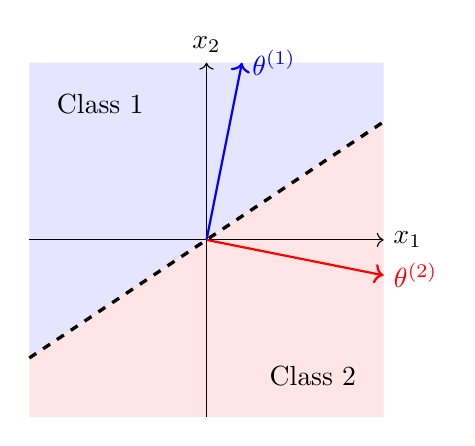
\begin{tikzpicture}[scale=0.75]
				\fill[blue!10] (-3,3) -- (-3,-2) -- (3,2) -- (3,3) -- cycle;
				\fill[red!10] (-3,-3) -- (-3,-2) -- (3,2) -- (3,-3) -- cycle;
				
				\draw[->] (-3,0) -- (3,0) node[right] {$x_1$};
				\draw[->] (0,-3) -- (0,3) node[above] {$x_2$};
				
				\draw[very thick, dashed] (-3,-2) -- (3,2);
				
				\draw[->, thick, blue] (0,0) -- (0.6,3) node[right] {$\theta^{(1)}$};
				\draw[->, thick, red] (0,0) -- (3,-0.6) node[right] {$\theta^{(2)}$};
				
				\node at (-1.8,2.3) {Class 1};
				\node at (1.8,-2.3) {Class 2};
			\end{tikzpicture}
		\end{center}
		
		\item[(iii)]
		\[
		\theta^{(1)}-\theta^{(2)}=[1,2]^T-[2,4]^T=[-1,-2]^T
		\]
		so the boundary is
		\[
		-x_1-2x_2=0
		\Rightarrow
		x_2=-\frac{1}{2}x_1.
		\]
		Class 1 occurs when \(-x_1-2x_2>0\), and class 2 occurs when \(-x_1-2x_2<0\).
		
		\begin{center}
			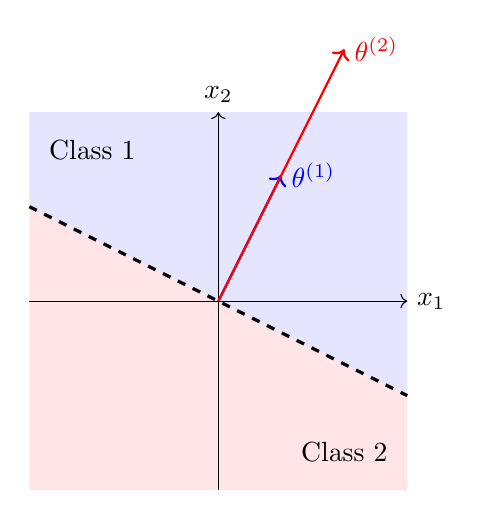
\begin{tikzpicture}[scale=0.8]
				\fill[blue!10] (-3,3) -- (-3,1.5) -- (3,-1.5) -- (3,3) -- cycle;
				\fill[red!10] (-3,-3) -- (-3,1.5) -- (3,-1.5) -- (3,-3) -- cycle;
				
				\draw[->] (-3,0) -- (3,0) node[right] {$x_1$};
				\draw[->] (0,-3) -- (0,3) node[above] {$x_2$};
				
				\draw[very thick, dashed] (-3,1.5) -- (3,-1.5);
				
				\draw[->, thick, blue] (0,0) -- (1,2) node[right] {$\theta^{(1)}$};
				\draw[->, thick, red] (0,0) -- (2,4) node[right] {$\theta^{(2)}$};
				
				\node at (-2,2.4) {Class 1};
				\node at (2,-2.4) {Class 2};
			\end{tikzpicture}
		\end{center}
		
	\end{enumerate}
	
	\newpage
	
	\noindent\textbf{4(b)} For each case given in 4(a), plug-in the ideal input \(\mathbf{x}=\theta^{(1)}\) and compute the following:
	
	\begin{enumerate}[itemsep=8pt]
		
		\item[(i)] Calculate the two probabilities for this case.
		
		\item[(ii)] Apply the probability rule to see what happens. Do you get the correct result?
		
	\end{enumerate}
	
	\noindent\textbf{Solution}
	
	For each case, use
	\[
	s_k(\mathbf{x})=(\theta^{(k)})^T\mathbf{x},
	\qquad
	\hat{p}_k=\frac{e^{s_k}}{e^{s_1}+e^{s_2}}.
	\]
	
	\begin{enumerate}[itemsep=4pt]
		
		\item[(i)] For \(\mathbf{x}=\theta^{(1)}=[1,2]^T\):
		\[
		s_1=5,\qquad s_2=3
		\]
		\[
		\hat{p}_1=\frac{e^5}{e^5+e^3}\approx 0.881,
		\qquad
		\hat{p}_2=\frac{e^3}{e^5+e^3}\approx 0.119
		\]
		Since \(\hat{p}_1>\hat{p}_2\), the sample is classified as class 1, which is correct.
		
		\item[(ii)] For \(\mathbf{x}=\theta^{(1)}=[1,5]^T\):
		\[
		s_1=26,\qquad s_2=0
		\]
		\[
		\hat{p}_1=\frac{e^{26}}{e^{26}+e^0}\approx 1,
		\qquad
		\hat{p}_2=\frac{e^0}{e^{26}+e^0}\approx 0
		\]
		Since \(\hat{p}_1>\hat{p}_2\), the sample is classified as class 1, which is correct.
		
		\item[(iii)] For \(\mathbf{x}=\theta^{(1)}=[1,2]^T\):
		\[
		s_1=5,\qquad s_2=10
		\]
		\[
		\hat{p}_1=\frac{e^5}{e^5+e^{10}}\approx 0.0067,
		\qquad
		\hat{p}_2=\frac{e^{10}}{e^5+e^{10}}\approx 0.9933
		\]
		Since \(\hat{p}_2>\hat{p}_1\), the sample is classified as class 2, so the result is incorrect.
		
	\end{enumerate}
	
	\newpage
	
	\noindent\textbf{Problem \#5. Attention equations (10 points).}
	
	\noindent\textbf{5(a)} For the attention module, we first compute:
	
	\[
	q_i=x_iW^Q,
	\qquad
	k_j=x_jW^K,
	\qquad
	v_j=x_jW^V.
	\]
	
	Then, the score function is just a dot-product:
	
	\[
	\mathrm{score}(x_i,x_j)
	=
	\frac{q_i\cdot k_j}{\sqrt{d_k}}.
	\]
	
	The key concept here is that we relate queries to keys via a simple dot product between vectors. The standard equations produce row vectors of size \(1\times n\) where \(n\) is the number of elements in the flattened \(x_i,x_j\) vectors.
	
	Now, for this problem, we want to use Linear Algebra, where the dot product between two column vectors are given by:
	
	\[
	q_i\cdot k_j
	=
	q_i k_j^T.
	\]
	
	For transposition, recall the basic rules:
	
	\[
	(A_1A_2\cdots A_m)^T
	=
	A_m^TA_{m-1}^T\cdots A_2^TA_1^T
	\qquad
	\mathrm{and}
	\qquad
	(A^T)^T=A.
	\]
	
	Substitute the equation for \(k_j^T\) to show that:
	
	\[
	\mathrm{score}(x_i,x_j)
	=
	\frac{1}{\sqrt{d_k}}
	x_i
	\left(
	W^Q(W^K)^T
	\right)
	x_j^T.
	\]
	
	\noindent\textbf{Solution}
	
	Starting with
	
	\[
	\mathrm{score}(x_i,x_j)
	=
	\frac{q_i\cdot k_j}{\sqrt{d_k}},
	\qquad
	q_i\cdot k_j=q_i k_j^T
	\]
	
	and substituting
	
	\[
	q_i=x_iW^Q,
	\qquad
	k_j=x_jW^K,
	\]
	
	we obtain
	
	\[
	\mathrm{score}(x_i,x_j)
	=
	\frac{1}{\sqrt{d_k}}
	(x_iW^Q)k_j^T.
	\]
	
	Using the transpose rule,
	
	\[
	k_j^T
	=
	(x_jW^K)^T
	=
	(W^K)^T x_j^T.
	\]
	
	Therefore,
	
	\[
	q_i k_j^T
	=
	(x_iW^Q)\left((W^K)^T x_j^T\right)
	=
	x_i\left(W^Q(W^K)^T\right)x_j^T.
	\]
	
	Thus,
	
	\[
	\mathrm{score}(x_i,x_j)
	=
	\frac{1}{\sqrt{d_k}}
	x_i
	\left(
	W^Q(W^K)^T
	\right)
	x_j^T.
	\]
	
	\newpage
	
	\noindent\textbf{5(b)} Unlike our SoftMax example, where the inputs are multiplied against fixed vectors, both vectors in the product can change during inference. However, during inference, the weight matrices \(W^Q\) and \(W^K\) remain fixed to the values that were learned during training.
	
	Instead of using the scores to visualize varying relationships based on specific inputs, we can use the product matrix
	
	\[
	W = W^Q(W^K)^T
	\]
	
	to visualize permanent relationships based on the locations of the input tokens (e.g., the indices \(i,j\)). For the following examples, compute simplified expressions for \(\mathrm{score}(x_i,x_j)\):
	
	\begin{enumerate}[itemsep=8pt]
		
		\item[(i)] First row of \(W\) is zero.
		
		\item[(ii)] First column of \(W\) is zero.
		
	\end{enumerate}
	
	\noindent\textbf{Solution}
	
	Using the result from 5(a),
	
	\[
	\mathrm{score}(x_i,x_j)
	=
	\frac{1}{\sqrt{d_k}}x_iWx_j^T.
	\]
	
	Since \(x_iWx_j^T\) selects the \((i,j)\)-th entry of \(W\),
	
	\[
	\mathrm{score}(x_i,x_j)
	=
	\frac{1}{\sqrt{d_k}}W_{ij}.
	\]
	
	\begin{enumerate}[itemsep=4pt]
		
		\item[(i)] If the first row of \(W\) is zero, then
		
		\[
		W_{1j}=0
		\quad \text{for all } j.
		\]
		
		Therefore,
		
		\[
		\mathrm{score}(x_1,x_j)
		=
		\frac{1}{\sqrt{d_k}}W_{1j}
		=
		0
		\quad \text{for all } j.
		\]
		
		\item[(ii)] If the first column of \(W\) is zero, then
		
		\[
		W_{i1}=0
		\quad \text{for all } i.
		\]
		
		Therefore,
		
		\[
		\mathrm{score}(x_i,x_1)
		=
		\frac{1}{\sqrt{d_k}}W_{i1}
		=
		0
		\quad \text{for all } i.
		\]
		
	\end{enumerate}
	
	\newpage
	
	\noindent\textbf{Problem 6. Transformer architecture problem (35 points).}
	
	For this problem, you need to provide a system diagram that illustrates the connections between the components. Here are the rules:
	
	\begin{enumerate}[itemsep=8pt]
		
		\item[(i)] Use directional arrows to show connections. The beginning of the arrow denotes the input. The end arrow shows where the input is connected.
		
		\item[(ii)] Clearly identify the inputs to the entire system. They should be associated with the start of an arrow.
		
		\item[(iii)] Clearly identify the outputs of the entire system. They should be associated with an arrow ending.
		
		\item[(iv)] Clearly identify the connections of internal variables that appear in the code. This will help me assess that you understand the code.
		
		\item[(v)] Clearly identify skip connections with directional arrows.
		
		\item[(vi)] Label each component using the name of the function and the line number at which it appears in the code. This will help me clearly identify any mistakes that you may be making in the diagram.
		
		\item[(vii)] Treat external function calls as components. In other words, there is no need to go inside and describe the internal connections of external functions. Here, we say that a function is external if it belongs to another class. However, you must clearly identify the connections to the input variables and outputs that appear in the definitions of the functions.
		
		\item[(viii)] You need to describe connections of any internal functions that appear in the class that you are given.
		
		\item[(ix)] Use a simple rectangle to represent each component. Note that dropout needs to appear inside the component where it is applied. It is not a separate component.
		
	\end{enumerate}
	
	Here is the list of classes for which you need to draw a diagram:
	
	\begin{enumerate}[itemsep=6pt]
		
		\item[(a)] PatchEmbedding 
		(\href{https://colab.research.google.com/drive/1gFiqft0ngNU7nIxpqfbfJ94XhnSdju5u?usp=sharing}{Fixed\_16\_vision\_and\_multimodal\_transformers.ipynb})
		
		\item[(b)] TransformerEncoderLayer 
		(\href{https://colab.research.google.com/drive/1T1-v3hXGcXqsljqvuRmXmlGUBS7qYo_b?usp=sharing}{Part\_15\_transformers\_for\_nlp\_and\_chatbots.ipynb})
		
		\item[(c)] TransformerEncoder 
		(\href{https://colab.research.google.com/drive/1T1-v3hXGcXqsljqvuRmXmlGUBS7qYo_b?usp=sharing}{Part\_15\_transformers\_for\_nlp\_and\_chatbots.ipynb})
		
		\item[(d)] ViT 
		(\href{https://colab.research.google.com/drive/1gFiqft0ngNU7nIxpqfbfJ94XhnSdju5u?usp=sharing}{Fixed\_16\_vision\_and\_multimodal\_transformers.ipynb})
		
	\end{enumerate}
	
	\newpage
	
	\noindent\textbf{Solution}
	
	\begin{center}
		\textbf{(a) PatchEmbedding}
	\end{center}
	
	\begin{center}
		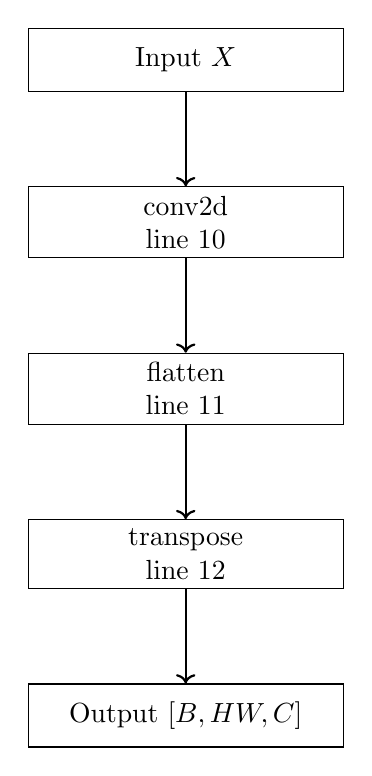
\begin{tikzpicture}[node distance=1.2cm,
			box/.style={draw, rectangle, minimum width=4cm, minimum height=0.8cm, align=center},
			arrow/.style={->, thick}]
			
			\node[box] (in) {Input \(X\)};
			\node[box, below=of in] (conv) {conv2d\\line 10};
			\node[box, below=of conv] (flat) {flatten\\line 11};
			\node[box, below=of flat] (trans) {transpose\\line 12};
			\node[box, below=of trans] (out) {Output \([B,HW,C]\)};
			
			\draw[arrow] (in) -- (conv);
			\draw[arrow] (conv) -- (flat);
			\draw[arrow] (flat) -- (trans);
			\draw[arrow] (trans) -- (out);
			
		\end{tikzpicture}
	\end{center}
	
	\begin{center}
		\textbf{(b) TransformerEncoderLayer}
	\end{center}
	
	\begin{center}
		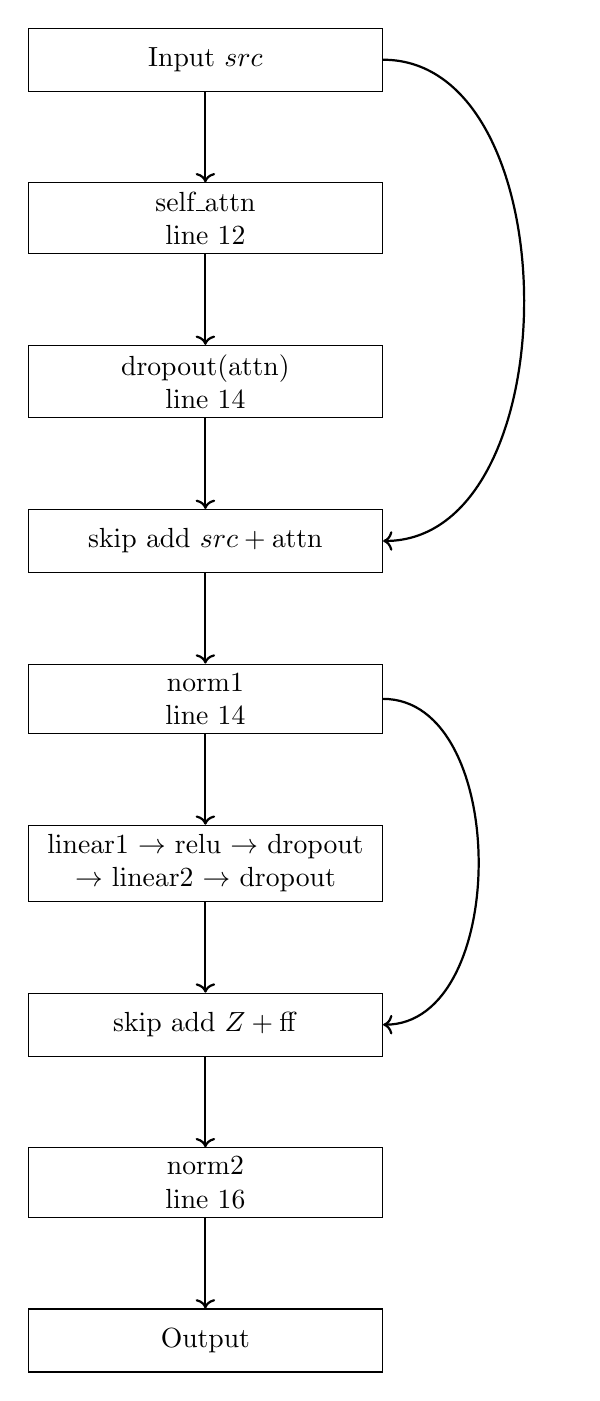
\begin{tikzpicture}[node distance=1.15cm,
			box/.style={draw, rectangle, minimum width=4.5cm, minimum height=0.8cm, align=center},
			arrow/.style={->, thick}]
			
			\node[box] (src) {Input \(src\)};
			\node[box, below=of src] (attn) {self\_attn\\line 12};
			\node[box, below=of attn] (drop1) {dropout(attn)\\line 14};
			\node[box, below=of drop1] (add1) {skip add \(src+\mathrm{attn}\)};
			\node[box, below=of add1] (norm1) {norm1\\line 14};
			\node[box, below=of norm1] (ff) {linear1 $\rightarrow$ relu $\rightarrow$ dropout\\$\rightarrow$ linear2 $\rightarrow$ dropout};
			\node[box, below=of ff] (add2) {skip add \(Z+\mathrm{ff}\)};
			\node[box, below=of add2] (norm2) {norm2\\line 16};
			\node[box, below=of norm2] (out) {Output};
			
			\draw[arrow] (src) -- (attn);
			\draw[arrow] (attn) -- (drop1);
			\draw[arrow] (drop1) -- (add1);
			\draw[arrow] (add1) -- (norm1);
			\draw[arrow] (norm1) -- (ff);
			\draw[arrow] (ff) -- (add2);
			\draw[arrow] (add2) -- (norm2);
			\draw[arrow] (norm2) -- (out);
			
			\draw[arrow] (src.east) to[out=0,in=0] (add1.east);
			\draw[arrow] (norm1.east) to[out=0,in=0] (add2.east);
			
		\end{tikzpicture}
	\end{center}
	
	\begin{center}
		\textbf{(c) TransformerEncoder}
	\end{center}
	
	\begin{center}
		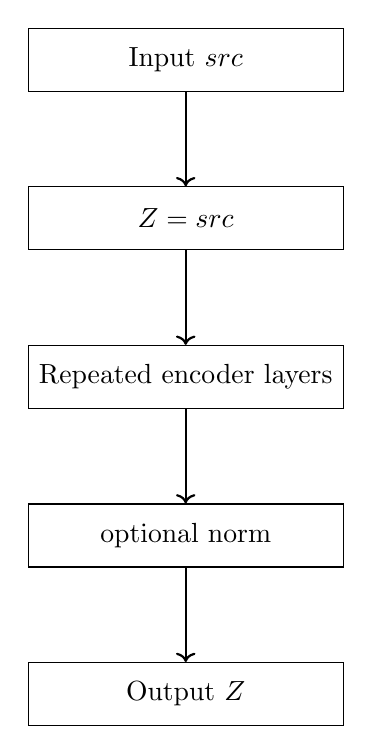
\begin{tikzpicture}[node distance=1.2cm,
			box/.style={draw, rectangle, minimum width=4cm, minimum height=0.8cm, align=center},
			arrow/.style={->, thick}]
			
			\node[box] (src) {Input \(src\)};
			\node[box, below=of src] (init) {\(Z=src\)};
			\node[box, below=of init] (layers) {Repeated encoder layers};
			\node[box, below=of layers] (norm) {optional norm};
			\node[box, below=of norm] (out) {Output \(Z\)};
			
			\draw[arrow] (src) -- (init);
			\draw[arrow] (init) -- (layers);
			\draw[arrow] (layers) -- (norm);
			\draw[arrow] (norm) -- (out);
			
		\end{tikzpicture}
	\end{center}
	
	\begin{center}
		\textbf{(d) ViT}
	\end{center}
	
	\begin{center}
		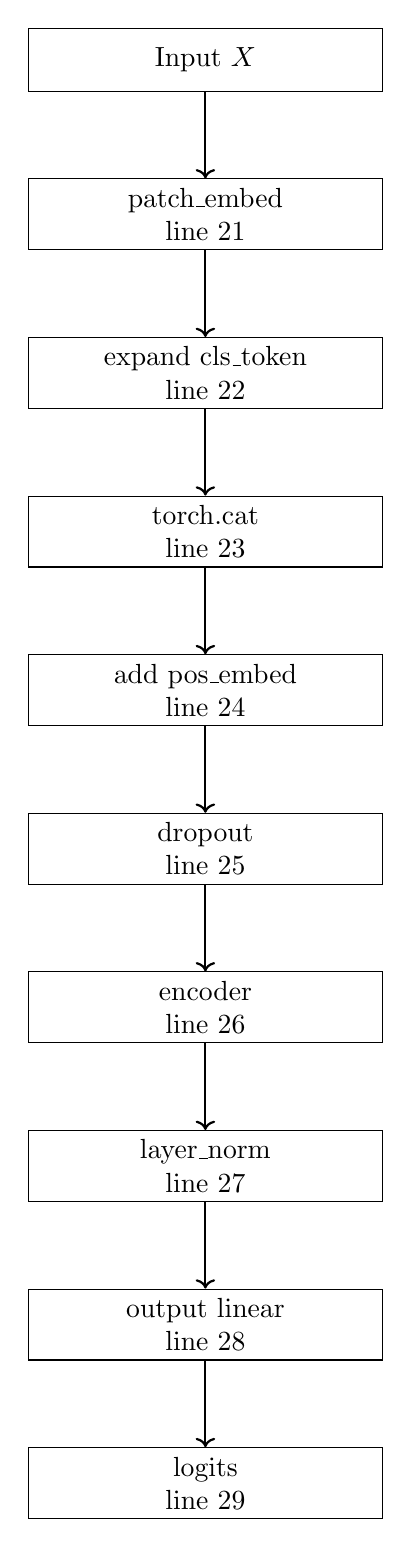
\begin{tikzpicture}[node distance=1.1cm,
			box/.style={draw, rectangle, minimum width=4.5cm, minimum height=0.8cm, align=center},
			arrow/.style={->, thick}]
			
			\node[box] (in) {Input \(X\)};
			\node[box, below=of in] (patch) {patch\_embed\\line 21};f
			\node[box, below=of patch] (cls) {expand cls\_token\\line 22};
			\node[box, below=of cls] (cat) {torch.cat\\line 23};
			\node[box, below=of cat] (pos) {add pos\_embed\\line 24};
			\node[box, below=of pos] (drop) {dropout\\line 25};
			\node[box, below=of drop] (enc) {encoder\\line 26};
			\node[box, below=of enc] (ln) {layer\_norm\\line 27};
			\node[box, below=of ln] (linear) {output linear\\line 28};
			\node[box, below=of linear] (out) {logits\\line 29};
			
			\draw[arrow] (in) -- (patch);
			\draw[arrow] (patch) -- (cls);
			\draw[arrow] (cls) -- (cat);
			\draw[arrow] (cat) -- (pos);
			\draw[arrow] (pos) -- (drop);
			\draw[arrow] (drop) -- (enc);
			\draw[arrow] (enc) -- (ln);
			\draw[arrow] (ln) -- (linear);
			\draw[arrow] (linear) -- (out);
			
		\end{tikzpicture}
	\end{center}
	
\end{document}